\section{Introduction}
\label{sec:Introduction}

\subsection{Background}
Generating content for computer games, CGI effects, feature films, print media, or Role-playing games is a significant bottleneck in terms of effort and resources. A typical game contains many thousands of audio files, images, textures, and 3D models. Procedurally generated content provides a cost-effective alternative to the manual creation of models, textures, images, and sound assets and can expand playability beyond what is otherwise possible. The video game ``No Man's Sky,'' for example, was released in 2016 and relied on procedural asset generation to create over 18 quintillion planets each of which has a unique ecosystem composed of flora and fauna. Such a scale is, of course, beyond the reach of any manually created system. Figure \ref{Screenshot NoManSky} is a screenshot of a planetary terrain region of ``No Man's Sky.''

\begin{figure}[htb]
\centering
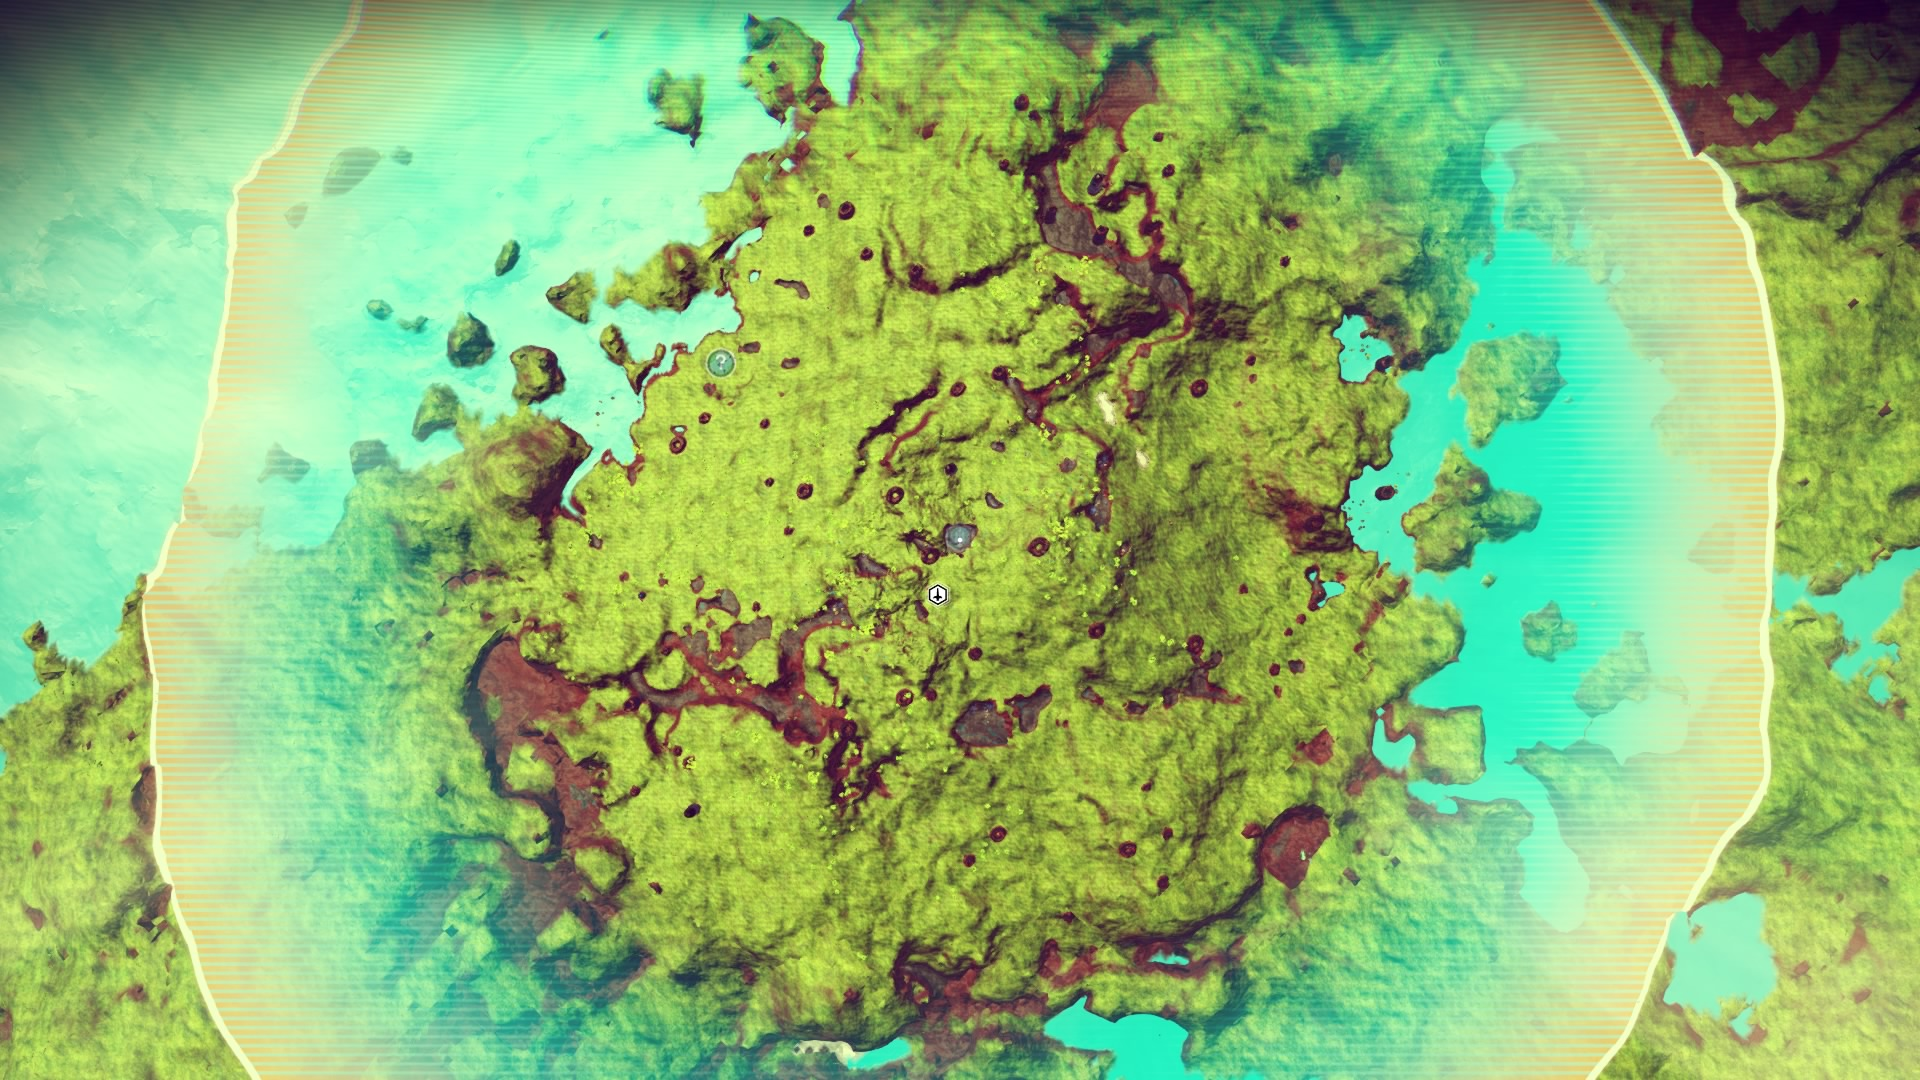
\includegraphics[width=\textwidth]{section01/assets/screenshot_NoManSky.jpg}
\caption[A screenshot of a planetary terrain region of ``No Man's Sky'']{\label{Screenshot NoManSky}A screenshot of a planetary terrain region of ``No Man's Sky''}
\end{figure}

\subsection{Similar Systems}
% The goal of this project is to automatically generate city maps for use in Role-playing games or world building narratives.
\subsubsection{Minecraft}
``Minecraft'' is a computer game that can produce massive worlds that are chock-full of little details, like elaborate cliff faces and waterfalls. Moreover, it relies on procedural generation, which automatically creates environments and objects that are at once random but guided by rules that maintain a consistent logic. Mountains are always rocky and sprinkled with snow, for example, while the low lands are typically full of grass and trees. Figure \ref{Screenshot Minecraft} is a screenshot of ``Minecraft.''

\begin{figure}[htb]
\centering
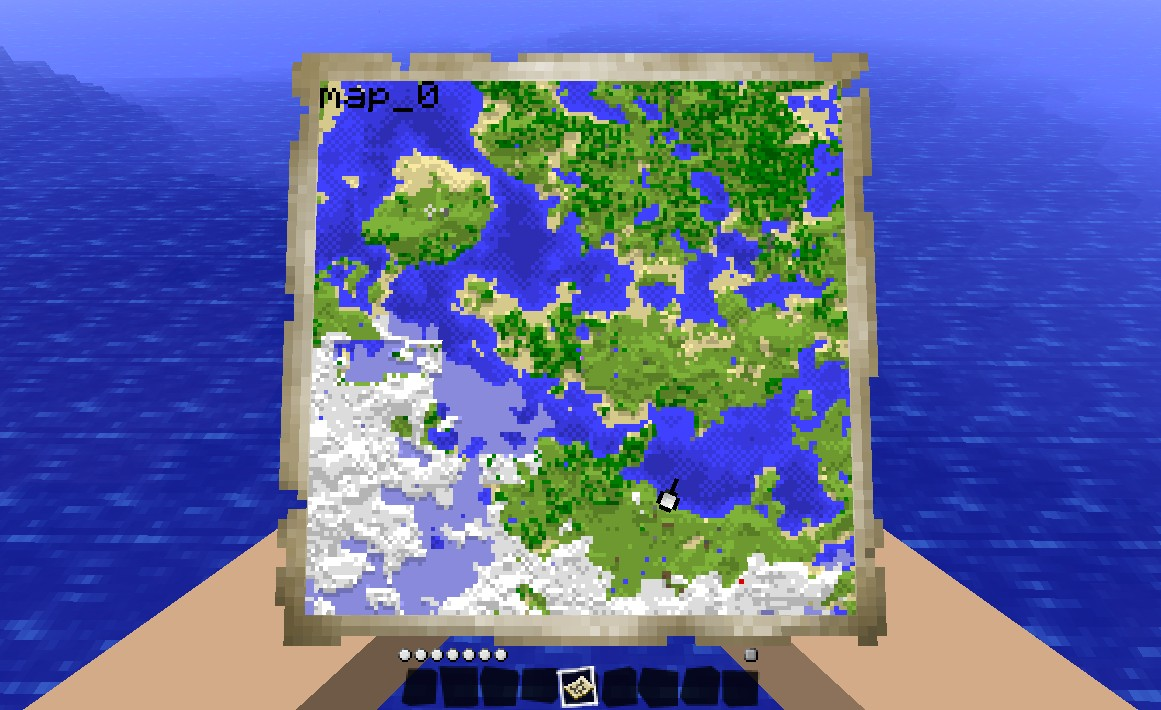
\includegraphics[width=\textwidth]{section01/assets/screenshot_Minecraft.jpg}
\caption[A screenshot of ``Minecraft'']{\label{Screenshot Minecraft}A screenshot of ``Minecraft''}
\end{figure}

\subsubsection{Medieval Fantasy City Generator(MFCG)}
The ``Medieval Fantasy City Generator(MFCG)'' is a web application. This application generates a random medieval city layout of a requested size: small, medium or large, which is made up of different types of regions, and the generation method is rather arbitrary. Furthermore, many elements are provided for the user to add to the city, such as farm fields, citadel, plaza, temple, river, coast and so on. Because of the premise of medieval fantasy, the map always includes the walls and castle, but the user can decide whether to display them. It allows the user to edit the map to modify some unsatisfying places using the warp tool. The author also mentioned that the goal of the application is to produce a nice looking map, not an accurate model of a city. Finally, the user can save the map as an image in the ``png'' or ``svg'' format by using the export feature if he is satisfied with the map. Figure \ref{Screenshot MFCG} is a screenshot of MFCG.

\begin{figure}[htb]
\centering
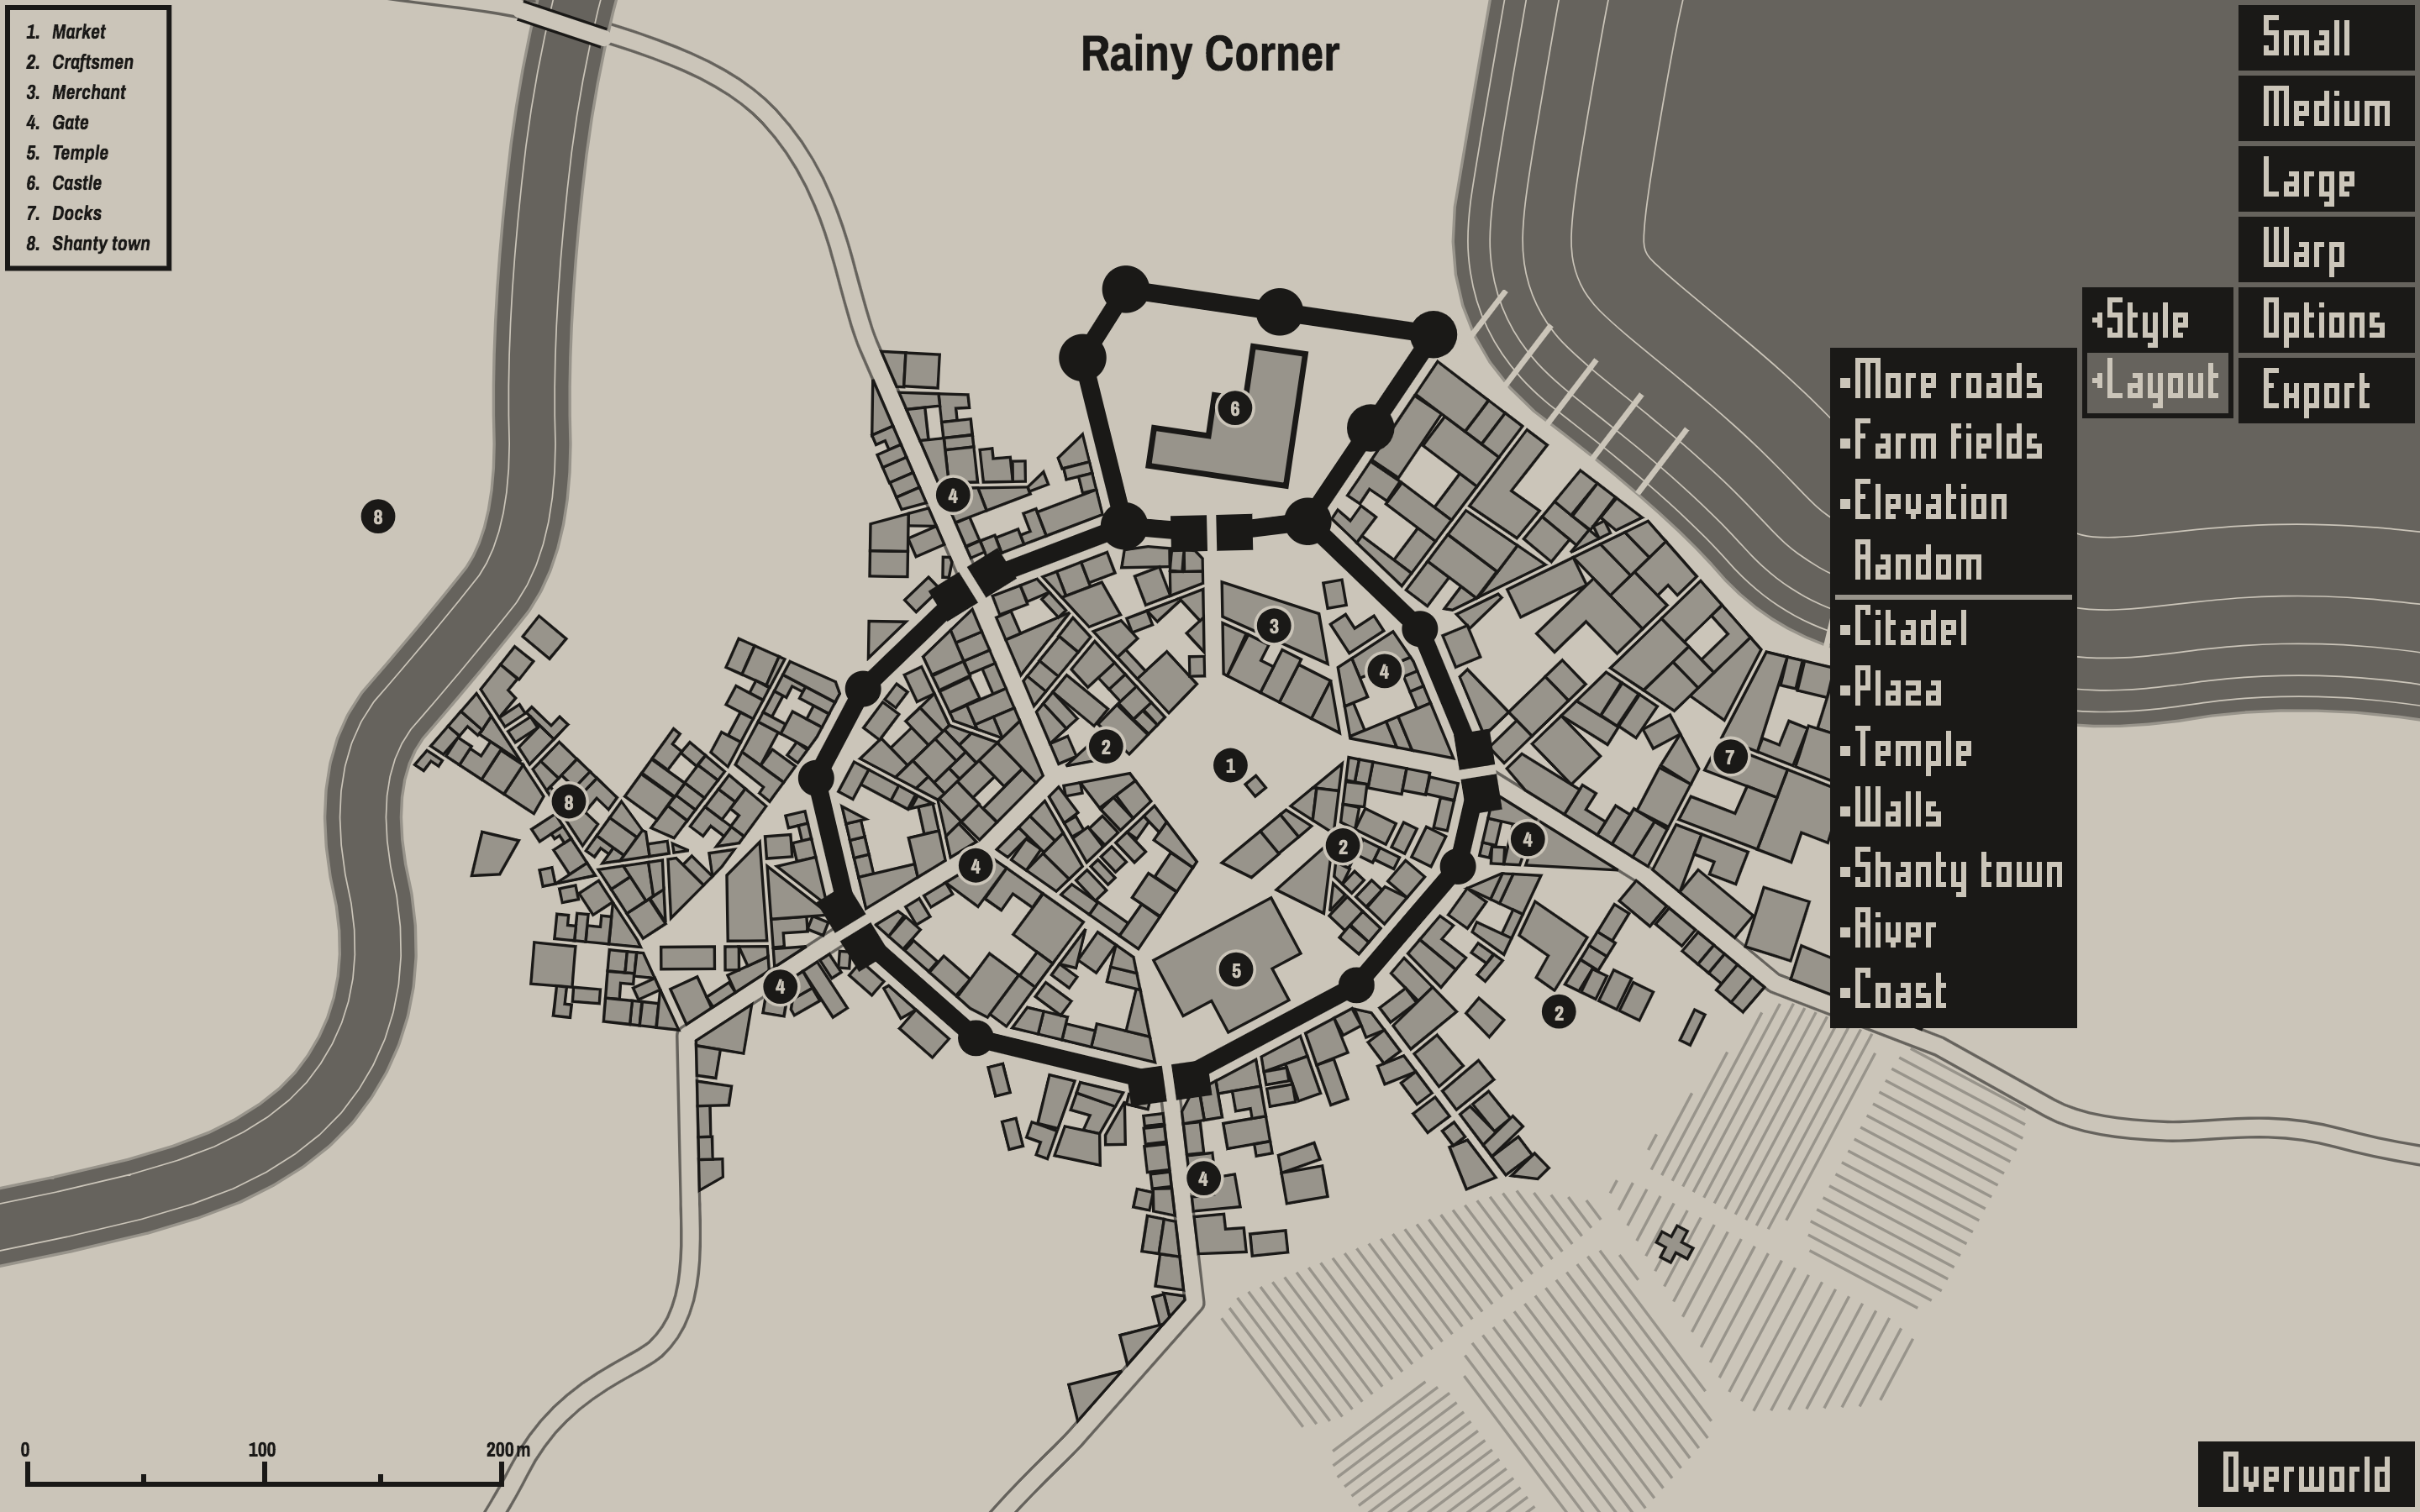
\includegraphics[width=\textwidth]{section01/assets/screenshot_MFCG.png}
\caption[A screenshot of the Medieval Fantasy City Generator]{\label{Screenshot MFCG}A screenshot of the Medieval Fantasy City Generator}
\end{figure}

\subsubsection{Azgaar's Fantasy Map Generator(FMG)}
The ``Azgaar's Fantasy Map Generator(FMG)'' is another similar system, which is a large scale system. The size of the map made by FMG varies from western Europe to the world continent, not just an island, but a random fantasy map represents a pseudo-medieval world. Just like the real world, the map generated by FMG has the feature that the continent is always surrounded by the ocean and will never touch the border of the map. Although it is a random map, it is still based on real-world rules. While its most prominent feature is that the user can choose the type of map he likes, which provides the following 5 map types: political, cultural, height, biomes and pure landmass. It also supports user-defined map type, and the user can add additional layers on existing map layers: rivers, temperature, and population. Also, it allows the user to annotate and edit the map using various such editors: layout, style, template, scale, countries, or cultural. It also supports exporting the map in the ``png'' or ``svg'' format, but unlike the previous application, if the user wants to come back to edit the map in the future, he can save it in the ``map'' format. Figure \ref{Screenshot FMG} is a screenshot of FMG.

\begin{figure}[htb]
\centering
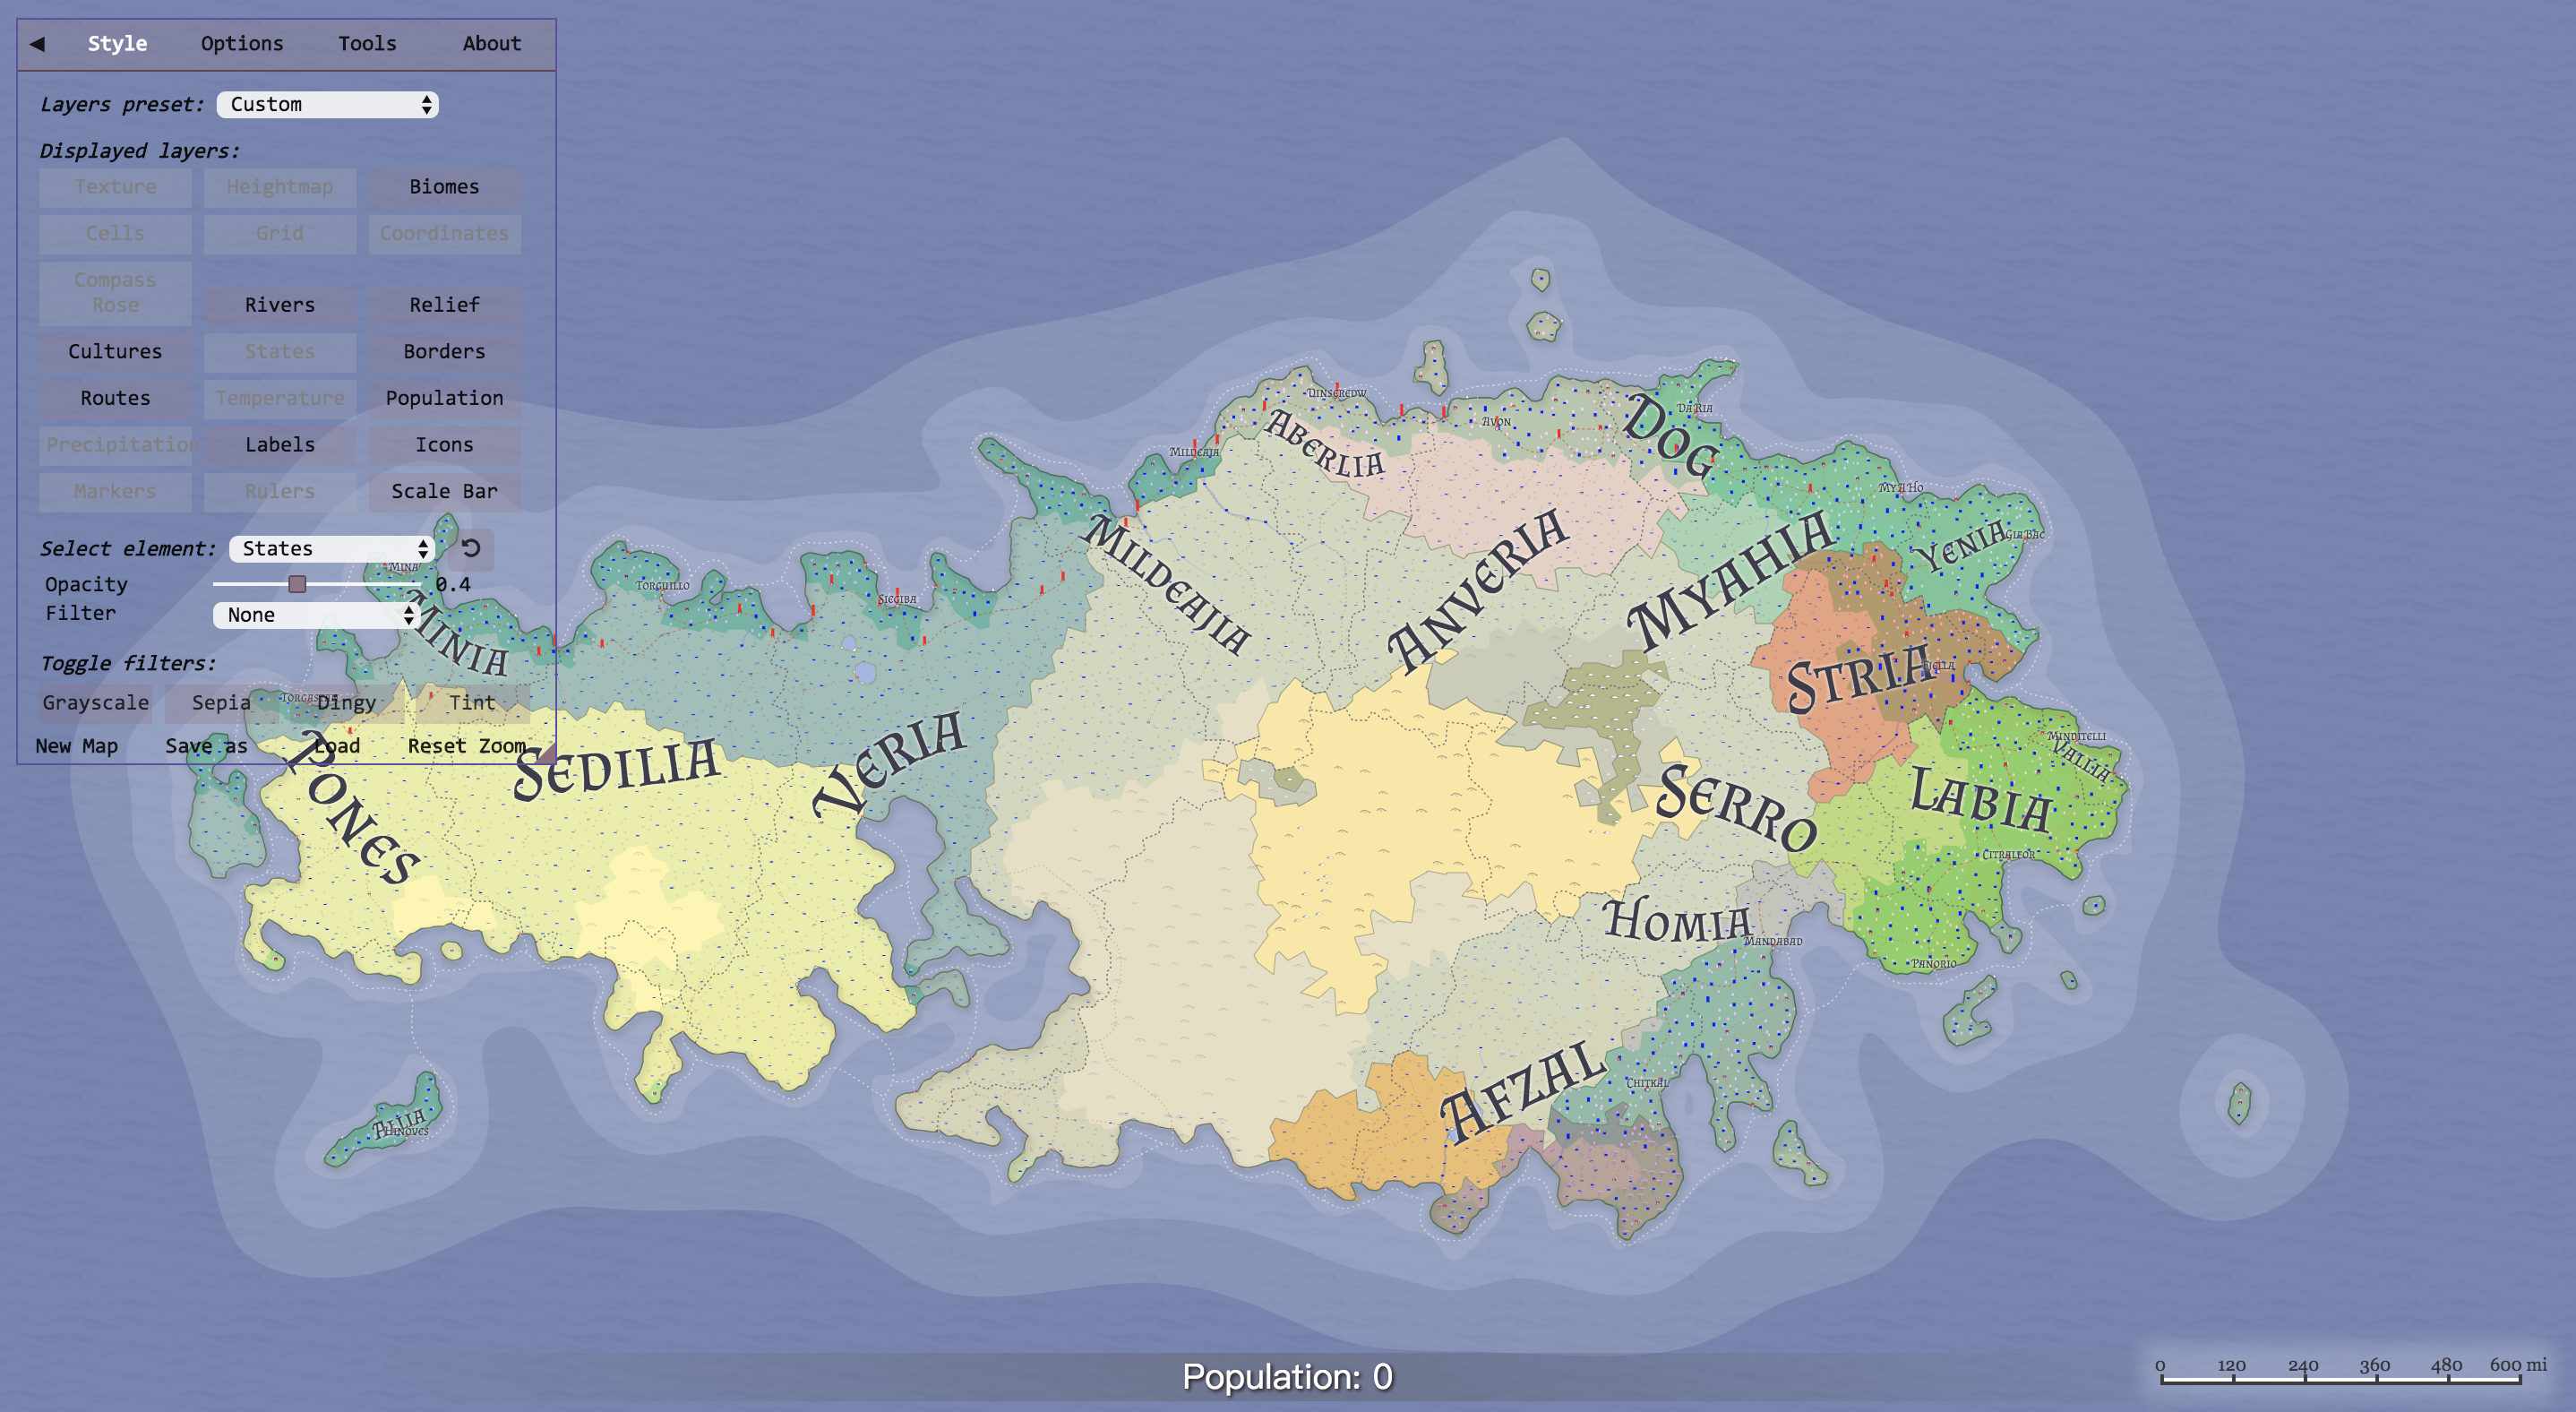
\includegraphics[width=\textwidth]{section01/assets/screenshot_FMG.png}
\caption[A screenshot of the Azgaar's Fantasy Map Generator]{\label{Screenshot FMG}A screenshot of the Azgaar's Fantasy Map Generator}
\end{figure}

\subsection{Project Goal}
The goal of this project is to automatically generate city maps for use in Role-playing games or Worldbuilding narratives. While the ultimate goal of this project is to procedurally replicate maps of a quality similar to the best cartographic hand-created maps by expert artists, we expect to obtain a modest approximation to the desired level of quality. Our system will have the essential features, such as: allowing the user to annotate or edit, supporting the user to export the map as an image in the ``png'' or ``svg'' format, allowing the user to save it to the database and restore it from the server. To achieve these goals, we provide the following operations and obey these rules:
\begin{itemize}
  \item The user should use the given tool to draw the map
  \item The user manually creates water, lands, and walls
  \item The map procedurally generates districts, buildings, streets, and street names
\end{itemize}
